% !TeX spellcheck = fr_FR

% TODO: Replace scan images with clean text where possible

\documentclass[a4paper, 10pt]{report}

\usepackage[french]{babel}
\usepackage[T1]{fontenc}

\usepackage{amsmath, amssymb, amsfonts}

\usepackage{hyperref}
\usepackage{geometry}

\usepackage{xcolor}
\usepackage{graphicx}

\usepackage{fancyhdr}
\usepackage{lastpage}

\usepackage{enumitem}

\geometry{
	a4paper,
	left=25mm,
	right=25mm,
	top=35mm,
	bottom=25mm,
	headsep=5mm,
	headheight=20mm,
}

\definecolor{solution}{HTML}{E5E4E2}
\providecommand{\abs}[1]{\lvert#1\rvert}
\providecommand{\norm}[1]{\lVert#1\rVert}

\begin{document}
	
	\renewcommand{\headrule}{%
		\vspace{-4pt}\hrulefill
		\raisebox{-6.8pt}{\ 
\includegraphics[height=5mm]{../../icon.png}}
		\hrulefill
	}	
	\pagestyle{fancy}
	\fancyhf{}
	
	\fancyhead[L]{\small \slshape Automne 2024}
	\fancyhead[C]{\Large \bfseries Logique et Théorie des Ensembles\\
		Série 06-B}
	\fancyhead[R]{\small Buff Mathias}
	\fancyfoot[L]{
		\small Source files available at:
		\href{https://github.com/MathiasBuff/bsc-math}
		{github.com/MathiasBuff/bsc-math}
	}
	\fancyfoot[R]{
		\small Page \thepage
		\hspace{1pt} /
		\pageref*{LastPage}
	}
	
	
	\noindent
	\textbf{Exercice 1.} Déterminer quelles sont les fonctions
	injectives, surjectives, et bijections parmi la liste suivante.
	Justifier vos affirmations.
	\begin{enumerate}[label=\arabic*.]
		\item $f : \begin{aligned}
			&\mathbb{R} \setminus \{0\} &&\to \mathbb{R} \setminus \{0\}\\
			&x &&\mapsto \tfrac{1}{x}
		\end{aligned}$
		%
		\item $g : \begin{aligned}
			&\mathbb{N} \setminus \{0, 1\} &&\to \mathbb{N}\\
			&n &&\mapsto \text{le plus petit nombre premier
			divisant}\ n
		\end{aligned}$
		%
		\item Pour $A \subset E$,
		$h: \begin{aligned}
			&\mathcal{P}(E) &&\to \mathcal{P}(A)\\
			&X &&\mapsto X \cap A
		\end{aligned}$
		(la réponse dépend de $A$).
	\end{enumerate}
	
	\colorbox{solution}
	{\begin{minipage}{0.9\textwidth}
		\begin{enumerate}[label=\arabic*.]
			\item $f$ est injective : Soient $x, x' \in \mathbb{R}$,
			alors $\frac{1}{x} = \frac{1}{x'} \implies
				\frac{1}{1/x} = \frac{1}{1/x'} \implies x = x'$.\\
			$f$ est surjective : Soit $y \in \mathbb{R}$, alors
			$x := \frac{1}{y} \in \mathbb{R}$ satisfait $y = f(x)$.\\
			$f$ est donc bijective, avec $f^{-1}: y \mapsto \frac{1}{y}$.
			%
			\vspace{6pt}
			%
			\item $g$ n'est pas injective, car $g(2) = g(4)$.\\
			$g$ n'est pas surjective, car $4 \in \mathbb{N}$
			n'est pas premier, donc
			$\forall x \in \mathbb{N}\setminus\{0, 1\}, f(x) \neq 4$.
			%
			\vspace{6pt}
			%
			\item \begin{itemize}[leftmargin=20mm]
				\item[Si $A=E$ :] $\forall X \subset E$, $X \cap E = X$,
				donc $h$ est alors la fonction identité dans
				$\mathcal{P}(E)$,\\
				$h: \begin{aligned}
					&\mathcal{P}(E) &&\to \mathcal{P}(E)\\
					&X &&\mapsto X
				\end{aligned}$\\
				Elle est donc bijective, et $h^{-1} = h$.
				%
				\item[Si $A \neq E$ :] Comme $\mathcal{P}(A) \subset
					\mathcal{P}(E),\ \text{alors}\
					\forall Y \in \mathcal{P}(A), Y \in \mathcal{P}(E)\
					\text{et}\ h(Y) = Y$,\\
					donc $h$ est surjective.\\
					De plus, $\forall X \subset E \setminus A \in
						\mathcal{P}(E), h(X) = \emptyset$, donc $h$
					n'est pas injective.
			\end{itemize}
			%
			\vspace{6pt}
			%
			On en conclut que $h$ est surjective indépendamment de $A$,
			mais qu'elle n'est injective que si $A = E$.
		\end{enumerate}
	\end{minipage}}

	\newpage
	
	\fancyhf{}
	\renewcommand{\headrule}
	{\rule{\textwidth}{0pt}}
	\fancyfoot[R]{
		\small Page \thepage
		\hspace{1pt} /
		\pageref*{LastPage}
	}
		
	\noindent
	\textbf{Exercice 2.} (Fonctions caractéristiques $\chi_A$).\\
	Soient $E$ un ensemble et $A \subset E$. La fonction
	caractéristique de A est définie par
	\[\chi_A : \begin{aligned}
		&E &&\to \{0, 1\}\\
		&x &&\mapsto \left\{
		\begin{aligned}
			&1 & &\text{si}\ x \in A\\
			&0 & &\text{sinon.}
		\end{aligned}
		\right.
	\end{aligned}\]
	
	\begin{enumerate}[label=\arabic*.]
		\item Montrer que deux ensembles sont égaux si et seulement
		si ils ont la même fonction caractéristique.
		
		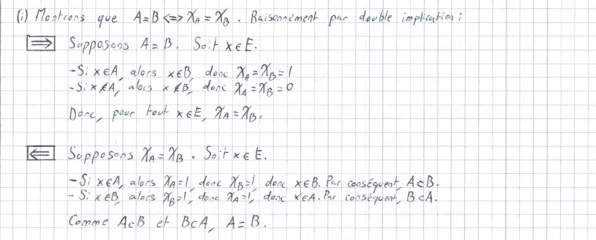
\includegraphics{ex02-1.jpg}
		%
		\item Que peut-on dire sur $A$ et $B$ si
		$\chi_A(x) \leq \chi_B(x)$ pour tout $x \in E$ ?
		
		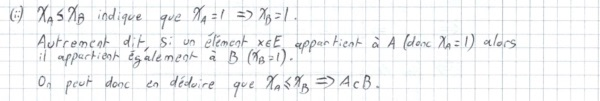
\includegraphics{ex02-2.jpg}
		%
		\item Montrer que $\chi_{A \cap B} = \chi_A \chi_B$,
		$\chi_{A^C} = 1 - \chi_A$ et
		$\chi_{A \cup B} = \chi_A + \chi_B - \chi_A \chi_B$.
		
		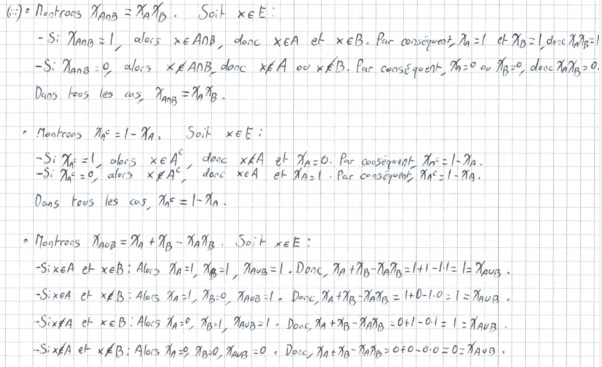
\includegraphics{ex02-3.jpg}
		%
		\item Montrer que les formules de De Morgan pour $(A \cup B)^C$
		et $(A \cap B)^C$ en utilisant les fonctions caractéristiques.
		
		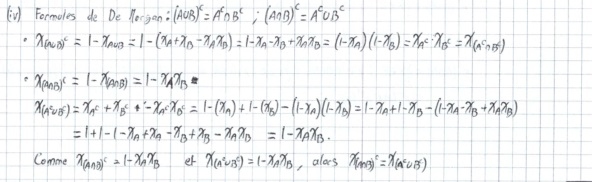
\includegraphics{ex02-4.jpg}
	\end{enumerate}
		
	\vspace{5mm}
	\noindent
	\textbf{Exercice 3.} Soient $f : E \to F$ et $g : F \to G$ deux
	fonctions.
	\begin{enumerate}[label=\arabic*.]
		\item On suppose que $g \circ f$ est injective.\\
		Montrer que $f$ est injective et trouver un exemple pour
		lequel $g$ ne l'est pas.
		%
		\item On suppose que $g \circ f$ est surjective.\\
		Montrer que $g$ est surjective et trouver un exemple pour
		lequel $f$ ne l'est pas.
		%
		\item Montrer que $g \circ f$ bijective n'implique pas que
		$f$ et $g$ soient bijectives.
	\end{enumerate}
	
	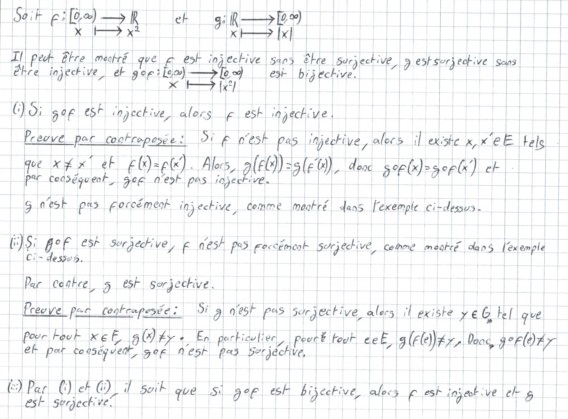
\includegraphics{ex03.jpg}
	
	\newpage
	
	\noindent
	\textbf{Exercice 4.} Montrer que si $f$ est une application de $E$
	dans $F$ et $(E_i)_{i \in I}$ est une famille d'ensembles inclus
	dans $E$,
	\[f\Big(\bigcup\limits_{i \in I}E_i\Big)
			= \bigcup\limits_{i \in I}f(E_i)\]
	De plus, montrer que si $f$ est injective,
	\[f\Big(\bigcap\limits_{i \in I}E_i\Big)
			= \bigcap\limits_{i \in I}f(E_i)\]
	Que peut-on dire si $f$ n'est pas injective ?
	
	\colorbox{solution}
	{\begin{minipage}{0.9\textwidth}
		\[\begin{split}
			f\Big(\bigcup\limits_{i \in I}E_i\Big)
			&= f(\{x \in E \mid \exists i \in I, x \in E_i\})\\
			&= \{f(x) \in F \mid \exists i \in I, x \in E_i\}\\
			&= \{f(x) \in F \mid \exists i \in I, f(x) \in f(E_i)\}\\
			&= \bigcup\limits_{i \in I}f(E_i)
		\end{split}\]
		
		Sans considération particulière de $f$:\\
		Soit $x \in \bigcap\limits_{i \in I}E_i$, alors
		$\forall i \in I, x \in E_i$ donc $f(x) \in f(E_i)$, et par
		conséquent $f(x) \in \bigcap\limits_{i \in I}f(E_i)$.\\
		\begin{equation}\label{eq:1}
			\text{Ainsi},\quad f\Big(\bigcap\limits_{i \in I}E_i\Big)
			\subset \bigcap\limits_{i \in I}f(E_i)
		\end{equation}
			
		De plus, supposons $f$ injective:\\
		Soit $y := f(x) \in \bigcap\limits_{i \in I}f(E_i)$, alors
		$\forall i \in I, y \in f(E_i)$ et comme $f$ injective
		$x \in E_i$, alors $x \in \bigcap\limits_{i \in I}E_i$
		et $f(x) \in f(\bigcap\limits_{i \in I}E_i)$.\\
		\begin{equation}\label{eq:2}
			\text{Ainsi},\quad \bigcap\limits_{i \in I}f(E_i)
			\subset f\Big(\bigcap\limits_{i \in I}E_i\Big)
		\end{equation}
		
		Par \eqref{eq:1} et \eqref{eq:2}, on conclut que si $f$ est
		injective, $\displaystyle f\Big(\bigcap\limits_{i \in I}E_i\Big)
			= \bigcap\limits_{i \in I}f(E_i)$.
		
	\end{minipage}}
	
\end{document}
